\section{Supporting displays and full-cell estimates}
\label{app:displays}
\begin{figure}[!htbp]
\centering
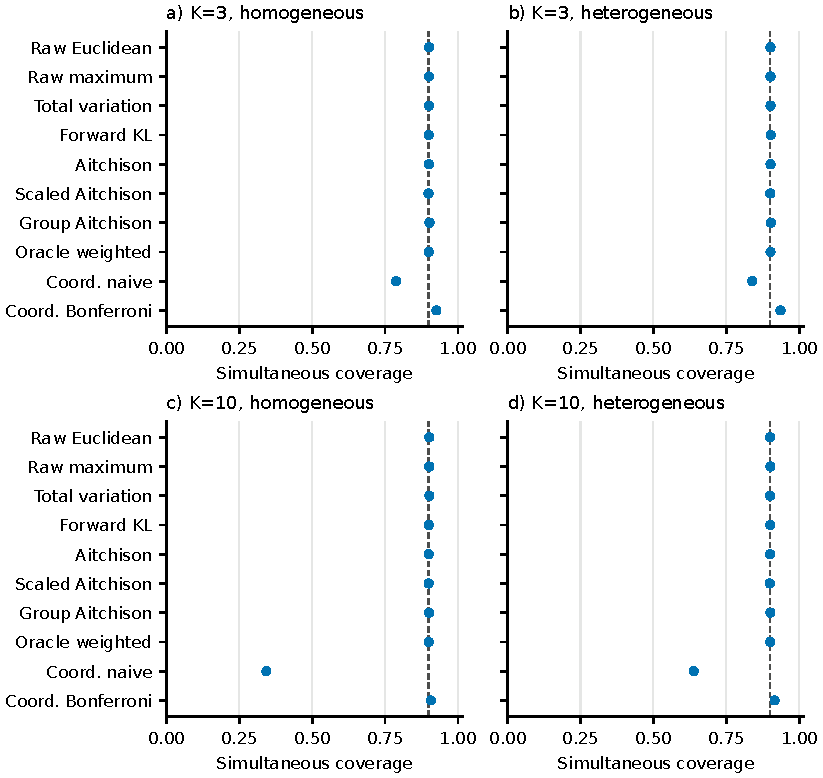
\includegraphics[width=\linewidth]{figures/joint_coverage.pdf}
\caption[Joint coverage across dimensions and noise settings]{\textbf{Joint response coverage under iid sampling.} Dots are means across 100 independent train/calibration/test replications; bars are pointwise 95\% $t$ intervals for these means, not simultaneous bands or intervals for a single calibrated run. Each replication uses 1000 training and 499 calibration observations and 5000 test observations per environment. The dashed line marks nominal $1-\alpha=0.90$. The target is the entire observed composition, not a class label. ``Coord. naive'' calibrates each coordinate at $\alpha$ and is a negative control; ``Coord. Bonferroni'' uses $\alpha/K$. Raw Euclidean and maximum regions are intersected with the simplex; Aitchison denotes the Euclidean norm of clr differences. The oracle weighted method uses unit weights under iid sampling. TV is exactly raw maximum at $K=3$ and is distinct at $K=10$; KL is forward $D_{\rm KL}(y\Vert\hat\mu)$.
}
\label{fig:joint_coverage}
\end{figure}
\begin{figure}[p]
\centering
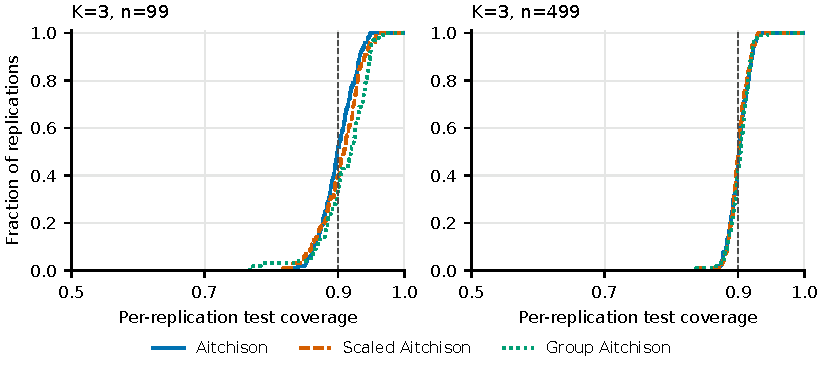
\includegraphics[width=\linewidth]{figures/replication_variability.pdf}
\caption[Variation across calibrated datasets]{\textbf{Mean validity does not guarantee every calibrated run.} Empirical cumulative distributions of finite-test joint coverage across 100 independent datasets in the iid heterogeneous $K=3$ setting, for calibration sizes 99 and 499. Global, training-only scaled and observed-group Aitchison methods share datasets within each replication. Each plotted coverage uses 5000 independent test responses conditional on its fitted and calibrated predictor; it still contains finite-test noise. The dashed line marks 0.90. These distributions and their empirical lower tails are descriptive, not certified probabilities of population conditional validity.
}
\label{fig:replication_variability}
\end{figure}
\begin{figure}[p]
\centering
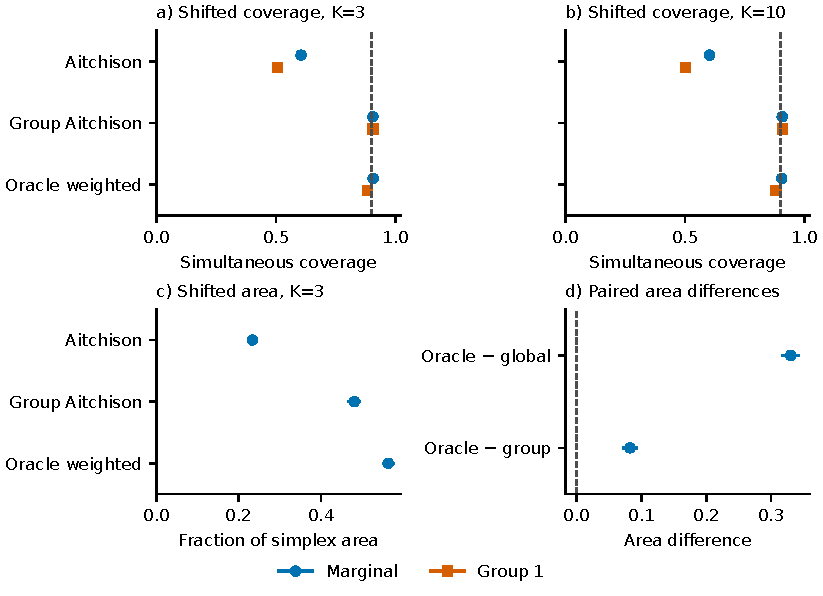
\includegraphics[width=\linewidth]{figures/oracle_shift.pdf}
\caption[Known-ratio oracle and group calibration under shift]{\textbf{Known-ratio weighting under the controlled mixture shift.} Heterogeneous mechanism, calibration size 499; test group-1 probability changes from 0.2 to 0.8 with within-group laws fixed. Panels (a,b) show shifted marginal and higher-noise-group joint coverage; (c) shows shifted-feature-averaged Euclidean simplex-area fractions at $K=3$; (d) shows within-seed paired oracle-minus-global and oracle-minus-group area differences. Dots/bars are means/pointwise 95\% $t$ intervals across independent dataset replications, not simultaneous bands. Oracle weights use exact generator density ratios with test weight at infinity. This does not evaluate learned ratios or arbitrary-shift robustness. Area needs the coverage context in (a,b).
}
\label{fig:oracle_shift}
\end{figure}
\begin{figure}[p]
\centering
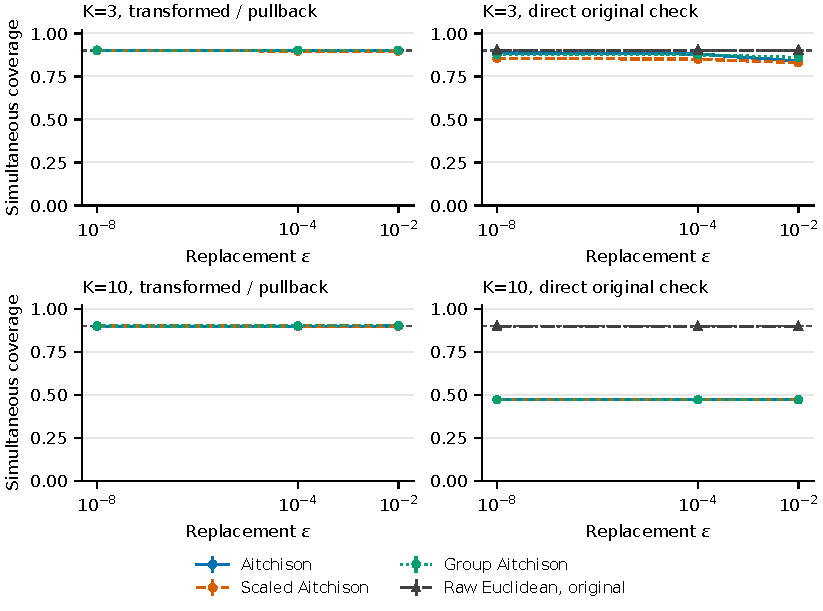
\includegraphics[width=\linewidth]{figures/boundary_targets.pdf}
\caption[Transformed and original boundary targets]{\textbf{Replacement changes the coverage target.} Exact zeros arise by censoring components below 0.025 and reclosing. The fixed transform is $T_\epsilon(y)_j=\max(y_j,\epsilon)/\sum_l\max(y_l,\epsilon)$. Left: clr methods calibrate and test on $T_\epsilon(Y)$. These same values and intervals exactly equal original-response coverage of the inverse-image region $\{y:T_\epsilon(y)\in C_\epsilon(x)\}$ by event identity; this is not another simulation. Right: those same finite clr regions are tested against original $Y$, rejecting boundary points, while the raw Euclidean reference separately calibrates and tests on original $Y$. All fits use transformed training responses. Dots are means and bars pointwise 95\% $t$ intervals across 50 independent datasets, with 1000 training, 499 calibration and 5000 iid test observations each. The same original datasets are reused across replacement values. The dashed line marks 0.90; the original-clr check has no nominal guarantee. The right-panel diagnostic is a different region from the left-panel inverse image. Replacement does not inherently prevent coverage of original zeros. No inverse-image area was estimated, and this censoring test does not establish structural-zero performance.
}
\label{fig:boundary_targets}
\end{figure}
\clearpage
\begin{table}[t]
\centering
\caption[Finite-test lower-tail diagnostics]{\textbf{Finite-test lower tails across calibrated datasets.} Heterogeneous iid cells; 100 independent replications each. The coverage 10th percentile is descriptive; the fraction of replications with 5000-test-point coverage below .85 has a pointwise 95\% Wilson interval. These are not certified population conditional-coverage probabilities because finite-test noise remains. Full diagnostics and infinite-region counts are in \texttt{tables/calibration\_diagnostics.csv}.
}
\label{tab:tails}
{\small\begin{tabular}{rrlrr}
\toprule
$K$ & $n$ & Method & Coverage 10th percentile & Fraction below .85 [95\% CI] \\
\midrule
3 & 99 & Aitchison & 0.864 & 0.02 [0.01, 0.07] \\
3 & 99 & Group Aitchison & 0.869 & 0.04 [0.02, 0.10] \\
3 & 99 & Scaled Aitchison & 0.861 & 0.06 [0.03, 0.12] \\
3 & 499 & Aitchison & 0.883 & 0.00 [0.00, 0.04] \\
3 & 499 & Group Aitchison & 0.884 & 0.01 [0.00, 0.05] \\
3 & 499 & Scaled Aitchison & 0.884 & 0.01 [0.00, 0.05] \\
10 & 99 & Aitchison & 0.858 & 0.05 [0.02, 0.11] \\
10 & 99 & Group Aitchison & 0.871 & 0.05 [0.02, 0.11] \\
10 & 99 & Scaled Aitchison & 0.867 & 0.06 [0.03, 0.12] \\
10 & 499 & Aitchison & 0.884 & 0.00 [0.00, 0.04] \\
10 & 499 & Group Aitchison & 0.882 & 0.00 [0.00, 0.04] \\
10 & 499 & Scaled Aitchison & 0.879 & 0.00 [0.00, 0.04] \\
\bottomrule
\end{tabular}
}
\end{table}
\clearpage
\begin{table}[p]
\centering
\caption[Prior-work score paired area contrasts]{\textbf{Source-driven score controls under a shared fitted predictor.} $K=3$, calibration size 499; paired within-seed area differences with pointwise 95\% $t$ intervals over 100 independent datasets. Negative values favor the first score only for the chosen uniform Euclidean simplex-area measure; judge them with subgroup and shifted coverage, not alone. Intervals including zero leave the ordering unresolved. TV is exactly raw maximum at $K=3$, including the zero paired differences shown here; these are not independent geometries. KL is forward $D_{\rm KL}(y\Vert\hat\mu)$. These controls were requested from permitted prior work after core results were inspected, before their own outcomes were known; they compare scores, not the prior study full fitted pipeline. Candidate-resolution diagnostics and all other cells are in \texttt{tables/area\_precision.csv} and \texttt{tables/paired\_method\_estimates.csv}.
}
\label{tab:prior_area}
{\small\begin{tabular}{llrr}
\toprule
Mechanism & Area difference & IID [95\% CI] & Shifted [95\% CI] \\
\midrule
homogeneous & TV $-$ Euclidean & -0.0027 [-0.0041, -0.0013] & -0.0025 [-0.0038, -0.0011] \\
homogeneous & TV $-$ Maximum & 0.0000 [0.0000, 0.0000] & 0.0000 [0.0000, 0.0000] \\
homogeneous & TV $-$ Aitchison & 0.0576 [0.0544, 0.0608] & 0.0620 [0.0589, 0.0651] \\
homogeneous & KL $-$ Euclidean & -0.0476 [-0.0493, -0.0459] & -0.0482 [-0.0498, -0.0465] \\
homogeneous & KL $-$ Maximum & -0.0448 [-0.0466, -0.0431] & -0.0457 [-0.0474, -0.0439] \\
homogeneous & KL $-$ Aitchison & 0.0128 [0.0104, 0.0151] & 0.0163 [0.0142, 0.0185] \\
heterogeneous & TV $-$ Euclidean & -0.0013 [-0.0031, 0.0005] & -0.0010 [-0.0027, 0.0007] \\
heterogeneous & TV $-$ Maximum & 0.0000 [0.0000, 0.0000] & 0.0000 [0.0000, 0.0000] \\
heterogeneous & TV $-$ Aitchison & -0.0222 [-0.0296, -0.0148] & -0.0125 [-0.0190, -0.0060] \\
heterogeneous & KL $-$ Euclidean & -0.0158 [-0.0197, -0.0120] & -0.0184 [-0.0220, -0.0147] \\
heterogeneous & KL $-$ Maximum & -0.0145 [-0.0181, -0.0109] & -0.0174 [-0.0208, -0.0139] \\
heterogeneous & KL $-$ Aitchison & -0.0367 [-0.0423, -0.0312] & -0.0298 [-0.0347, -0.0250] \\
\bottomrule
\end{tabular}
}
\end{table}
\clearpage
\noindent\textbf{Finite ranks and ties.} Each row uses 20,000 independent trials. Rank is $\lceil(n+1)(1-\alpha)\rceil$; $\infty$ denotes the whole-domain fallback. Theory is exact expected coverage including conservative Bernoulli ties. Test intervals are 95\% Wilson; calibration coverage (CDF at the threshold) has a pointwise 95\% $t$ interval for its trial mean. Variance checks and seeds remain in \texttt{tables/rank\_checks.csv}.

{\small\begin{longtable}{rrlrrrr}
\toprule
$n$ & $\alpha$ & Scores & Rank & Theory & Test [95\% CI] & Calibration [95\% CI] \\
\midrule
\endhead
2 & 0.05 & bernoulli & $\infty$ & 1.000 & 1.0000 [0.9998, 1.0000] & 1.000 [1.000, 1.000] \\
9 & 0.05 & bernoulli & $\infty$ & 1.000 & 1.0000 [0.9998, 1.0000] & 1.000 [1.000, 1.000] \\
19 & 0.05 & bernoulli & 19 & 1.000 & 1.0000 [0.9998, 1.0000] & 1.000 [1.000, 1.000] \\
99 & 0.05 & bernoulli & 95 & 1.000 & 1.0000 [0.9998, 1.0000] & 1.000 [1.000, 1.000] \\
499 & 0.05 & bernoulli & 475 & 1.000 & 1.0000 [0.9998, 1.0000] & 1.000 [1.000, 1.000] \\
2 & 0.1 & bernoulli & $\infty$ & 1.000 & 1.0000 [0.9998, 1.0000] & 1.000 [1.000, 1.000] \\
9 & 0.1 & bernoulli & 9 & 0.999 & 0.9991 [0.9986, 0.9995] & 0.999 [0.999, 0.999] \\
19 & 0.1 & bernoulli & 18 & 1.000 & 1.0000 [0.9997, 1.0000] & 1.000 [1.000, 1.000] \\
99 & 0.1 & bernoulli & 90 & 1.000 & 1.0000 [0.9998, 1.0000] & 1.000 [1.000, 1.000] \\
499 & 0.1 & bernoulli & 450 & 1.000 & 1.0000 [0.9998, 1.0000] & 1.000 [1.000, 1.000] \\
2 & 0.2 & bernoulli & $\infty$ & 1.000 & 1.0000 [0.9998, 1.0000] & 1.000 [1.000, 1.000] \\
9 & 0.2 & bernoulli & 8 & 0.990 & 0.9896 [0.9881, 0.9909] & 0.990 [0.989, 0.991] \\
19 & 0.2 & bernoulli & 16 & 0.999 & 0.9990 [0.9985, 0.9994] & 0.999 [0.999, 0.999] \\
99 & 0.2 & bernoulli & 80 & 1.000 & 1.0000 [0.9998, 1.0000] & 1.000 [1.000, 1.000] \\
499 & 0.2 & bernoulli & 400 & 1.000 & 1.0000 [0.9998, 1.0000] & 1.000 [1.000, 1.000] \\
2 & 0.05 & uniform & $\infty$ & 1.000 & 1.0000 [0.9998, 1.0000] & 1.000 [1.000, 1.000] \\
9 & 0.05 & uniform & $\infty$ & 1.000 & 1.0000 [0.9998, 1.0000] & 1.000 [1.000, 1.000] \\
19 & 0.05 & uniform & 19 & 0.950 & 0.9511 [0.9480, 0.9540] & 0.950 [0.949, 0.951] \\
99 & 0.05 & uniform & 95 & 0.950 & 0.9489 [0.9458, 0.9519] & 0.950 [0.950, 0.950] \\
499 & 0.05 & uniform & 475 & 0.950 & 0.9492 [0.9460, 0.9521] & 0.950 [0.950, 0.950] \\
2 & 0.1 & uniform & $\infty$ & 1.000 & 1.0000 [0.9998, 1.0000] & 1.000 [1.000, 1.000] \\
9 & 0.1 & uniform & 9 & 0.900 & 0.8979 [0.8936, 0.9020] & 0.899 [0.898, 0.900] \\
19 & 0.1 & uniform & 18 & 0.900 & 0.9002 [0.8959, 0.9042] & 0.900 [0.899, 0.901] \\
99 & 0.1 & uniform & 90 & 0.900 & 0.8976 [0.8934, 0.9018] & 0.900 [0.899, 0.900] \\
499 & 0.1 & uniform & 450 & 0.900 & 0.9001 [0.8959, 0.9042] & 0.900 [0.900, 0.900] \\
2 & 0.2 & uniform & $\infty$ & 1.000 & 1.0000 [0.9998, 1.0000] & 1.000 [1.000, 1.000] \\
9 & 0.2 & uniform & 8 & 0.800 & 0.8023 [0.7967, 0.8077] & 0.801 [0.799, 0.803] \\
19 & 0.2 & uniform & 16 & 0.800 & 0.7976 [0.7920, 0.8031] & 0.800 [0.799, 0.802] \\
99 & 0.2 & uniform & 80 & 0.800 & 0.8014 [0.7959, 0.8069] & 0.800 [0.800, 0.801] \\
499 & 0.2 & uniform & 400 & 0.800 & 0.7974 [0.7918, 0.8030] & 0.800 [0.800, 0.800] \\
\bottomrule
\end{longtable}
}
\clearpage
\subsection{All main-grid numeric panels}
The following panels retain all main dimension, calibration, noise and environment cells. Numerical source files also retain group 0 values, raw replication estimates and paired contrasts. Pointwise intervals do not imply simultaneous coverage guarantees across panels.
\begin{table}[!htbp]
\centering
\caption[Full cell: k10 n499 heterogeneous iid epsepsilon alpha0.1]{\textbf{Full-cell estimates: $K=10$, calibration size 499, heterogeneous.} IID test environment. All methods share 100 independent datasets. Brackets are pointwise 95\% $t$ intervals for replication means, not simultaneous bands. Area is the common Euclidean simplex fraction at $K=3$; -- means unmeasured at $K=10$. TV duplicates raw maximum at $K=3$; forward KL uses $y\Vert\hat\mu$. Group 1 is the prespecified higher-noise group in the heterogeneous mechanism. Full group-0 estimates and denominators are in \texttt{tables/all\_estimates.csv}.
}
{\small\begin{tabular}{lrrr}
\toprule
Method & Joint coverage & Group 1 coverage & Area fraction \\
\midrule
Raw Euclidean & 0.900 [0.898, 0.903] & 0.502 [0.489, 0.515] & -- \\
Raw maximum & 0.901 [0.898, 0.904] & 0.507 [0.494, 0.520] & -- \\
Total variation & 0.900 [0.898, 0.903] & 0.500 [0.487, 0.514] & -- \\
Forward KL & 0.901 [0.898, 0.903] & 0.502 [0.489, 0.514] & -- \\
Aitchison & 0.901 [0.898, 0.903] & 0.502 [0.489, 0.514] & -- \\
Scaled Aitchison & 0.899 [0.896, 0.902] & 0.894 [0.889, 0.899] & -- \\
Group Aitchison & 0.901 [0.898, 0.904] & 0.907 [0.901, 0.913] & -- \\
Oracle weighted & 0.901 [0.898, 0.903] & 0.502 [0.489, 0.514] & -- \\
Coord. naive & 0.638 [0.633, 0.643] & 0.011 [0.010, 0.012] & -- \\
Coord. Bonferroni & 0.916 [0.914, 0.918] & 0.582 [0.570, 0.593] & -- \\
\bottomrule
\end{tabular}
}
\end{table}
\begin{table}[p]
\centering
\caption[Full cell: k10 n499 heterogeneous shift epsepsilon alpha0.1]{\textbf{Full-cell estimates: $K=10$, calibration size 499, heterogeneous.} Controlled mixture-shift test environment. All methods share 100 independent datasets. Brackets are pointwise 95\% $t$ intervals for replication means, not simultaneous bands. Area is the common Euclidean simplex fraction at $K=3$; -- means unmeasured at $K=10$. TV duplicates raw maximum at $K=3$; forward KL uses $y\Vert\hat\mu$. Group 1 is the prespecified higher-noise group in the heterogeneous mechanism. Full group-0 estimates and denominators are in \texttt{tables/all\_estimates.csv}.
}
{\small\begin{tabular}{lrrr}
\toprule
Method & Joint coverage & Group 1 coverage & Area fraction \\
\midrule
Raw Euclidean & 0.601 [0.591, 0.611] & 0.501 [0.488, 0.514] & -- \\
Raw maximum & 0.605 [0.595, 0.615] & 0.507 [0.494, 0.519] & -- \\
Total variation & 0.601 [0.590, 0.611] & 0.501 [0.488, 0.513] & -- \\
Forward KL & 0.602 [0.592, 0.612] & 0.502 [0.490, 0.515] & -- \\
Aitchison & 0.603 [0.593, 0.612] & 0.503 [0.492, 0.515] & -- \\
Scaled Aitchison & 0.896 [0.892, 0.900] & 0.895 [0.890, 0.899] & -- \\
Group Aitchison & 0.907 [0.902, 0.911] & 0.908 [0.902, 0.914] & -- \\
Oracle weighted & 0.905 [0.899, 0.911] & 0.881 [0.874, 0.888] & -- \\
Coord. naive & 0.168 [0.167, 0.170] & 0.011 [0.011, 0.012] & -- \\
Coord. Bonferroni & 0.664 [0.655, 0.672] & 0.580 [0.568, 0.591] & -- \\
\bottomrule
\end{tabular}
}
\end{table}
\begin{table}[p]
\centering
\caption[Full cell: k10 n499 homogeneous iid epsepsilon alpha0.1]{\textbf{Full-cell estimates: $K=10$, calibration size 499, homogeneous.} IID test environment. All methods share 100 independent datasets. Brackets are pointwise 95\% $t$ intervals for replication means, not simultaneous bands. Area is the common Euclidean simplex fraction at $K=3$; -- means unmeasured at $K=10$. TV duplicates raw maximum at $K=3$; forward KL uses $y\Vert\hat\mu$. Group 1 is the prespecified higher-noise group in the heterogeneous mechanism. Full group-0 estimates and denominators are in \texttt{tables/all\_estimates.csv}.
}
{\small\begin{tabular}{lrrr}
\toprule
Method & Joint coverage & Group 1 coverage & Area fraction \\
\midrule
Raw Euclidean & 0.902 [0.899, 0.905] & 0.906 [0.903, 0.909] & -- \\
Raw maximum & 0.902 [0.899, 0.904] & 0.904 [0.901, 0.907] & -- \\
Total variation & 0.902 [0.899, 0.905] & 0.908 [0.905, 0.912] & -- \\
Forward KL & 0.900 [0.897, 0.903] & 0.906 [0.903, 0.909] & -- \\
Aitchison & 0.900 [0.897, 0.903] & 0.898 [0.894, 0.901] & -- \\
Scaled Aitchison & 0.900 [0.896, 0.903] & 0.895 [0.890, 0.899] & -- \\
Group Aitchison & 0.901 [0.898, 0.904] & 0.903 [0.897, 0.910] & -- \\
Oracle weighted & 0.900 [0.897, 0.903] & 0.898 [0.894, 0.901] & -- \\
Coord. naive & 0.343 [0.339, 0.347] & 0.318 [0.313, 0.322] & -- \\
Coord. Bonferroni & 0.907 [0.904, 0.910] & 0.893 [0.889, 0.897] & -- \\
\bottomrule
\end{tabular}
}
\end{table}
\begin{table}[p]
\centering
\caption[Full cell: k10 n499 homogeneous shift epsepsilon alpha0.1]{\textbf{Full-cell estimates: $K=10$, calibration size 499, homogeneous.} Controlled mixture-shift test environment. All methods share 100 independent datasets. Brackets are pointwise 95\% $t$ intervals for replication means, not simultaneous bands. Area is the common Euclidean simplex fraction at $K=3$; -- means unmeasured at $K=10$. TV duplicates raw maximum at $K=3$; forward KL uses $y\Vert\hat\mu$. Group 1 is the prespecified higher-noise group in the heterogeneous mechanism. Full group-0 estimates and denominators are in \texttt{tables/all\_estimates.csv}.
}
{\small\begin{tabular}{lrrr}
\toprule
Method & Joint coverage & Group 1 coverage & Area fraction \\
\midrule
Raw Euclidean & 0.904 [0.901, 0.906] & 0.904 [0.902, 0.907] & -- \\
Raw maximum & 0.902 [0.899, 0.905] & 0.902 [0.899, 0.905] & -- \\
Total variation & 0.907 [0.904, 0.910] & 0.908 [0.906, 0.911] & -- \\
Forward KL & 0.905 [0.902, 0.908] & 0.907 [0.904, 0.910] & -- \\
Aitchison & 0.899 [0.896, 0.902] & 0.899 [0.896, 0.902] & -- \\
Scaled Aitchison & 0.897 [0.892, 0.901] & 0.896 [0.891, 0.900] & -- \\
Group Aitchison & 0.903 [0.898, 0.909] & 0.904 [0.897, 0.911] & -- \\
Oracle weighted & 0.903 [0.898, 0.908] & 0.904 [0.899, 0.909] & -- \\
Coord. naive & 0.325 [0.321, 0.329] & 0.319 [0.315, 0.323] & -- \\
Coord. Bonferroni & 0.897 [0.894, 0.900] & 0.894 [0.890, 0.897] & -- \\
\bottomrule
\end{tabular}
}
\end{table}
\begin{table}[p]
\centering
\caption[Full cell: k10 n99 heterogeneous iid epsepsilon alpha0.1]{\textbf{Full-cell estimates: $K=10$, calibration size 99, heterogeneous.} IID test environment. All methods share 100 independent datasets. Brackets are pointwise 95\% $t$ intervals for replication means, not simultaneous bands. Area is the common Euclidean simplex fraction at $K=3$; -- means unmeasured at $K=10$. TV duplicates raw maximum at $K=3$; forward KL uses $y\Vert\hat\mu$. Group 1 is the prespecified higher-noise group in the heterogeneous mechanism. Full group-0 estimates and denominators are in \texttt{tables/all\_estimates.csv}.
}
{\small\begin{tabular}{lrrr}
\toprule
Method & Joint coverage & Group 1 coverage & Area fraction \\
\midrule
Raw Euclidean & 0.898 [0.892, 0.904] & 0.492 [0.462, 0.522] & -- \\
Raw maximum & 0.898 [0.892, 0.905] & 0.499 [0.470, 0.528] & -- \\
Total variation & 0.897 [0.891, 0.903] & 0.484 [0.454, 0.515] & -- \\
Forward KL & 0.898 [0.892, 0.904] & 0.490 [0.460, 0.520] & -- \\
Aitchison & 0.899 [0.893, 0.905] & 0.494 [0.463, 0.525] & -- \\
Scaled Aitchison & 0.899 [0.894, 0.905] & 0.893 [0.886, 0.900] & -- \\
Group Aitchison & 0.908 [0.903, 0.914] & 0.912 [0.898, 0.925] & -- \\
Oracle weighted & 0.899 [0.893, 0.905] & 0.494 [0.463, 0.525] & -- \\
Coord. naive & 0.621 [0.610, 0.633] & 0.012 [0.011, 0.014] & -- \\
Coord. Bonferroni & 0.917 [0.912, 0.922] & 0.593 [0.573, 0.614] & -- \\
\bottomrule
\end{tabular}
}
\end{table}
\begin{table}[p]
\centering
\caption[Full cell: k10 n99 heterogeneous shift epsepsilon alpha0.1]{\textbf{Full-cell estimates: $K=10$, calibration size 99, heterogeneous.} Controlled mixture-shift test environment. All methods share 100 independent datasets. Brackets are pointwise 95\% $t$ intervals for replication means, not simultaneous bands. Area is the common Euclidean simplex fraction at $K=3$; -- means unmeasured at $K=10$. TV duplicates raw maximum at $K=3$; forward KL uses $y\Vert\hat\mu$. Group 1 is the prespecified higher-noise group in the heterogeneous mechanism. Full group-0 estimates and denominators are in \texttt{tables/all\_estimates.csv}.
}
{\small\begin{tabular}{lrrr}
\toprule
Method & Joint coverage & Group 1 coverage & Area fraction \\
\midrule
Raw Euclidean & 0.593 [0.569, 0.618] & 0.492 [0.462, 0.522] & -- \\
Raw maximum & 0.599 [0.576, 0.623] & 0.500 [0.471, 0.529] & -- \\
Total variation & 0.588 [0.564, 0.613] & 0.486 [0.455, 0.516] & -- \\
Forward KL & 0.593 [0.569, 0.617] & 0.491 [0.462, 0.521] & -- \\
Aitchison & 0.595 [0.570, 0.619] & 0.493 [0.463, 0.523] & -- \\
Scaled Aitchison & 0.895 [0.889, 0.902] & 0.894 [0.888, 0.901] & -- \\
Group Aitchison & 0.912 [0.901, 0.923] & 0.913 [0.900, 0.927] & -- \\
Oracle weighted & 0.912 [0.900, 0.924] & 0.890 [0.875, 0.905] & -- \\
Coord. naive & 0.165 [0.161, 0.169] & 0.012 [0.011, 0.013] & -- \\
Coord. Bonferroni & 0.673 [0.656, 0.689] & 0.592 [0.572, 0.612] & -- \\
\bottomrule
\end{tabular}
}
\end{table}
\begin{table}[p]
\centering
\caption[Full cell: k10 n99 homogeneous iid epsepsilon alpha0.1]{\textbf{Full-cell estimates: $K=10$, calibration size 99, homogeneous.} IID test environment. All methods share 100 independent datasets. Brackets are pointwise 95\% $t$ intervals for replication means, not simultaneous bands. Area is the common Euclidean simplex fraction at $K=3$; -- means unmeasured at $K=10$. TV duplicates raw maximum at $K=3$; forward KL uses $y\Vert\hat\mu$. Group 1 is the prespecified higher-noise group in the heterogeneous mechanism. Full group-0 estimates and denominators are in \texttt{tables/all\_estimates.csv}.
}
{\small\begin{tabular}{lrrr}
\toprule
Method & Joint coverage & Group 1 coverage & Area fraction \\
\midrule
Raw Euclidean & 0.907 [0.901, 0.912] & 0.910 [0.905, 0.915] & -- \\
Raw maximum & 0.908 [0.902, 0.913] & 0.909 [0.904, 0.914] & -- \\
Total variation & 0.905 [0.900, 0.911] & 0.911 [0.906, 0.917] & -- \\
Forward KL & 0.903 [0.897, 0.908] & 0.909 [0.903, 0.914] & -- \\
Aitchison & 0.899 [0.893, 0.905] & 0.897 [0.891, 0.902] & -- \\
Scaled Aitchison & 0.898 [0.893, 0.904] & 0.893 [0.886, 0.899] & -- \\
Group Aitchison & 0.908 [0.903, 0.913] & 0.915 [0.902, 0.927] & -- \\
Oracle weighted & 0.899 [0.893, 0.905] & 0.897 [0.891, 0.902] & -- \\
Coord. naive & 0.343 [0.336, 0.350] & 0.322 [0.315, 0.329] & -- \\
Coord. Bonferroni & 0.910 [0.904, 0.915] & 0.896 [0.889, 0.903] & -- \\
\bottomrule
\end{tabular}
}
\end{table}
\begin{table}[p]
\centering
\caption[Full cell: k10 n99 homogeneous shift epsepsilon alpha0.1]{\textbf{Full-cell estimates: $K=10$, calibration size 99, homogeneous.} Controlled mixture-shift test environment. All methods share 100 independent datasets. Brackets are pointwise 95\% $t$ intervals for replication means, not simultaneous bands. Area is the common Euclidean simplex fraction at $K=3$; -- means unmeasured at $K=10$. TV duplicates raw maximum at $K=3$; forward KL uses $y\Vert\hat\mu$. Group 1 is the prespecified higher-noise group in the heterogeneous mechanism. Full group-0 estimates and denominators are in \texttt{tables/all\_estimates.csv}.
}
{\small\begin{tabular}{lrrr}
\toprule
Method & Joint coverage & Group 1 coverage & Area fraction \\
\midrule
Raw Euclidean & 0.908 [0.903, 0.914] & 0.909 [0.904, 0.914] & -- \\
Raw maximum & 0.908 [0.903, 0.913] & 0.908 [0.903, 0.913] & -- \\
Total variation & 0.909 [0.904, 0.914] & 0.911 [0.906, 0.916] & -- \\
Forward KL & 0.907 [0.901, 0.912] & 0.908 [0.903, 0.913] & -- \\
Aitchison & 0.898 [0.893, 0.904] & 0.899 [0.893, 0.905] & -- \\
Scaled Aitchison & 0.895 [0.889, 0.901] & 0.894 [0.888, 0.901] & -- \\
Group Aitchison & 0.912 [0.902, 0.922] & 0.914 [0.902, 0.927] & -- \\
Oracle weighted & 0.911 [0.902, 0.920] & 0.917 [0.908, 0.926] & -- \\
Coord. naive & 0.327 [0.320, 0.333] & 0.320 [0.314, 0.327] & -- \\
Coord. Bonferroni & 0.899 [0.893, 0.906] & 0.896 [0.889, 0.903] & -- \\
\bottomrule
\end{tabular}
}
\end{table}
\begin{table}[p]
\centering
\caption[Full cell: k3 n499 heterogeneous iid epsepsilon alpha0.1]{\textbf{Full-cell estimates: $K=3$, calibration size 499, heterogeneous.} IID test environment. All methods share 100 independent datasets. Brackets are pointwise 95\% $t$ intervals for replication means, not simultaneous bands. Area is the common Euclidean simplex fraction at $K=3$; -- means unmeasured at $K=10$. TV duplicates raw maximum at $K=3$; forward KL uses $y\Vert\hat\mu$. Group 1 is the prespecified higher-noise group in the heterogeneous mechanism. Full group-0 estimates and denominators are in \texttt{tables/all\_estimates.csv}.
}
{\small\begin{tabular}{lrrr}
\toprule
Method & Joint coverage & Group 1 coverage & Area fraction \\
\midrule
Raw Euclidean & 0.902 [0.899, 0.904] & 0.512 [0.499, 0.525] & 0.232 [0.222, 0.241] \\
Raw maximum & 0.902 [0.899, 0.905] & 0.512 [0.499, 0.525] & 0.230 [0.221, 0.240] \\
Total variation & 0.902 [0.899, 0.905] & 0.512 [0.499, 0.525] & 0.230 [0.221, 0.240] \\
Forward KL & 0.902 [0.900, 0.905] & 0.511 [0.499, 0.523] & 0.216 [0.208, 0.224] \\
Aitchison & 0.902 [0.899, 0.905] & 0.507 [0.493, 0.521] & 0.253 [0.243, 0.262] \\
Scaled Aitchison & 0.901 [0.898, 0.904] & 0.899 [0.894, 0.904] & 0.157 [0.150, 0.165] \\
Group Aitchison & 0.903 [0.900, 0.906] & 0.906 [0.901, 0.912] & 0.164 [0.155, 0.172] \\
Oracle weighted & 0.902 [0.899, 0.905] & 0.507 [0.493, 0.521] & 0.253 [0.243, 0.262] \\
Coord. naive & 0.839 [0.836, 0.842] & 0.324 [0.317, 0.331] & 0.090 [0.087, 0.092] \\
Coord. Bonferroni & 0.936 [0.934, 0.938] & 0.681 [0.671, 0.690] & 0.317 [0.308, 0.326] \\
\bottomrule
\end{tabular}
}
\end{table}
\begin{table}[p]
\centering
\caption[Full cell: k3 n499 heterogeneous shift epsepsilon alpha0.1]{\textbf{Full-cell estimates: $K=3$, calibration size 499, heterogeneous.} Controlled mixture-shift test environment. All methods share 100 independent datasets. Brackets are pointwise 95\% $t$ intervals for replication means, not simultaneous bands. Area is the common Euclidean simplex fraction at $K=3$; -- means unmeasured at $K=10$. TV duplicates raw maximum at $K=3$; forward KL uses $y\Vert\hat\mu$. Group 1 is the prespecified higher-noise group in the heterogeneous mechanism. Full group-0 estimates and denominators are in \texttt{tables/all\_estimates.csv}.
}
{\small\begin{tabular}{lrrr}
\toprule
Method & Joint coverage & Group 1 coverage & Area fraction \\
\midrule
Raw Euclidean & 0.608 [0.598, 0.618] & 0.510 [0.497, 0.522] & 0.222 [0.212, 0.231] \\
Raw maximum & 0.609 [0.598, 0.619] & 0.510 [0.498, 0.523] & 0.221 [0.211, 0.231] \\
Total variation & 0.609 [0.598, 0.619] & 0.510 [0.498, 0.523] & 0.221 [0.211, 0.231] \\
Forward KL & 0.608 [0.599, 0.618] & 0.510 [0.498, 0.522] & 0.203 [0.195, 0.212] \\
Aitchison & 0.605 [0.594, 0.616] & 0.506 [0.492, 0.519] & 0.233 [0.224, 0.243] \\
Scaled Aitchison & 0.898 [0.893, 0.902] & 0.896 [0.891, 0.901] & 0.462 [0.450, 0.474] \\
Group Aitchison & 0.905 [0.901, 0.910] & 0.906 [0.901, 0.911] & 0.481 [0.468, 0.494] \\
Oracle weighted & 0.907 [0.902, 0.911] & 0.883 [0.877, 0.889] & 0.563 [0.551, 0.575] \\
Coord. naive & 0.451 [0.445, 0.456] & 0.320 [0.314, 0.327] & 0.089 [0.086, 0.091] \\
Coord. Bonferroni & 0.744 [0.736, 0.751] & 0.679 [0.669, 0.689] & 0.308 [0.299, 0.317] \\
\bottomrule
\end{tabular}
}
\end{table}
\begin{table}[p]
\centering
\caption[Full cell: k3 n499 homogeneous iid epsepsilon alpha0.1]{\textbf{Full-cell estimates: $K=3$, calibration size 499, homogeneous.} IID test environment. All methods share 100 independent datasets. Brackets are pointwise 95\% $t$ intervals for replication means, not simultaneous bands. Area is the common Euclidean simplex fraction at $K=3$; -- means unmeasured at $K=10$. TV duplicates raw maximum at $K=3$; forward KL uses $y\Vert\hat\mu$. Group 1 is the prespecified higher-noise group in the heterogeneous mechanism. Full group-0 estimates and denominators are in \texttt{tables/all\_estimates.csv}.
}
{\small\begin{tabular}{lrrr}
\toprule
Method & Joint coverage & Group 1 coverage & Area fraction \\
\midrule
Raw Euclidean & 0.901 [0.898, 0.904] & 0.895 [0.891, 0.898] & 0.266 [0.261, 0.270] \\
Raw maximum & 0.901 [0.897, 0.904] & 0.898 [0.894, 0.901] & 0.263 [0.259, 0.268] \\
Total variation & 0.901 [0.897, 0.904] & 0.898 [0.894, 0.901] & 0.263 [0.259, 0.268] \\
Forward KL & 0.900 [0.897, 0.903] & 0.899 [0.896, 0.902] & 0.218 [0.214, 0.222] \\
Aitchison & 0.900 [0.897, 0.903] & 0.901 [0.898, 0.905] & 0.205 [0.201, 0.209] \\
Scaled Aitchison & 0.899 [0.896, 0.902] & 0.896 [0.891, 0.902] & 0.207 [0.203, 0.211] \\
Group Aitchison & 0.902 [0.899, 0.905] & 0.907 [0.902, 0.912] & 0.208 [0.204, 0.212] \\
Oracle weighted & 0.900 [0.897, 0.903] & 0.901 [0.898, 0.905] & 0.205 [0.201, 0.209] \\
Coord. naive & 0.788 [0.784, 0.791] & 0.805 [0.800, 0.809] & 0.153 [0.151, 0.155] \\
Coord. Bonferroni & 0.926 [0.923, 0.929] & 0.931 [0.928, 0.934] & 0.272 [0.267, 0.276] \\
\bottomrule
\end{tabular}
}
\end{table}
\begin{table}[p]
\centering
\caption[Full cell: k3 n499 homogeneous shift epsepsilon alpha0.1]{\textbf{Full-cell estimates: $K=3$, calibration size 499, homogeneous.} Controlled mixture-shift test environment. All methods share 100 independent datasets. Brackets are pointwise 95\% $t$ intervals for replication means, not simultaneous bands. Area is the common Euclidean simplex fraction at $K=3$; -- means unmeasured at $K=10$. TV duplicates raw maximum at $K=3$; forward KL uses $y\Vert\hat\mu$. Group 1 is the prespecified higher-noise group in the heterogeneous mechanism. Full group-0 estimates and denominators are in \texttt{tables/all\_estimates.csv}.
}
{\small\begin{tabular}{lrrr}
\toprule
Method & Joint coverage & Group 1 coverage & Area fraction \\
\midrule
Raw Euclidean & 0.896 [0.892, 0.899] & 0.894 [0.891, 0.897] & 0.254 [0.249, 0.258] \\
Raw maximum & 0.898 [0.895, 0.901] & 0.897 [0.894, 0.900] & 0.251 [0.247, 0.255] \\
Total variation & 0.898 [0.895, 0.901] & 0.897 [0.894, 0.900] & 0.251 [0.247, 0.255] \\
Forward KL & 0.899 [0.896, 0.902] & 0.898 [0.895, 0.901] & 0.206 [0.202, 0.209] \\
Aitchison & 0.900 [0.897, 0.903] & 0.899 [0.896, 0.902] & 0.189 [0.186, 0.193] \\
Scaled Aitchison & 0.896 [0.892, 0.900] & 0.895 [0.890, 0.900] & 0.190 [0.185, 0.194] \\
Group Aitchison & 0.905 [0.901, 0.909] & 0.905 [0.900, 0.911] & 0.195 [0.190, 0.200] \\
Oracle weighted & 0.904 [0.899, 0.908] & 0.905 [0.900, 0.909] & 0.194 [0.189, 0.198] \\
Coord. naive & 0.798 [0.795, 0.802] & 0.802 [0.798, 0.806] & 0.149 [0.147, 0.151] \\
Coord. Bonferroni & 0.930 [0.927, 0.933] & 0.931 [0.928, 0.934] & 0.262 [0.258, 0.266] \\
\bottomrule
\end{tabular}
}
\end{table}
\begin{table}[p]
\centering
\caption[Full cell: k3 n99 heterogeneous iid epsepsilon alpha0.1]{\textbf{Full-cell estimates: $K=3$, calibration size 99, heterogeneous.} IID test environment. All methods share 100 independent datasets. Brackets are pointwise 95\% $t$ intervals for replication means, not simultaneous bands. Area is the common Euclidean simplex fraction at $K=3$; -- means unmeasured at $K=10$. TV duplicates raw maximum at $K=3$; forward KL uses $y\Vert\hat\mu$. Group 1 is the prespecified higher-noise group in the heterogeneous mechanism. Full group-0 estimates and denominators are in \texttt{tables/all\_estimates.csv}.
}
{\small\begin{tabular}{lrrr}
\toprule
Method & Joint coverage & Group 1 coverage & Area fraction \\
\midrule
Raw Euclidean & 0.900 [0.894, 0.905] & 0.510 [0.487, 0.534] & 0.237 [0.218, 0.255] \\
Raw maximum & 0.900 [0.894, 0.905] & 0.511 [0.488, 0.534] & 0.235 [0.217, 0.253] \\
Total variation & 0.900 [0.894, 0.905] & 0.511 [0.488, 0.534] & 0.235 [0.217, 0.253] \\
Forward KL & 0.900 [0.895, 0.906] & 0.506 [0.481, 0.532] & 0.220 [0.203, 0.237] \\
Aitchison & 0.900 [0.894, 0.905] & 0.498 [0.473, 0.523] & 0.250 [0.234, 0.266] \\
Scaled Aitchison & 0.904 [0.898, 0.910] & 0.901 [0.894, 0.908] & 0.149 [0.139, 0.159] \\
Group Aitchison & 0.911 [0.904, 0.918] & 0.924 [0.913, 0.935] & 0.164 [0.153, 0.175] \\
Oracle weighted & 0.900 [0.894, 0.905] & 0.498 [0.473, 0.523] & 0.250 [0.234, 0.266] \\
Coord. naive & 0.833 [0.825, 0.840] & 0.328 [0.313, 0.344] & 0.095 [0.088, 0.102] \\
Coord. Bonferroni & 0.939 [0.935, 0.942] & 0.696 [0.678, 0.713] & 0.341 [0.324, 0.357] \\
\bottomrule
\end{tabular}
}
\end{table}
\begin{table}[p]
\centering
\caption[Full cell: k3 n99 heterogeneous shift epsepsilon alpha0.1]{\textbf{Full-cell estimates: $K=3$, calibration size 99, heterogeneous.} Controlled mixture-shift test environment. All methods share 100 independent datasets. Brackets are pointwise 95\% $t$ intervals for replication means, not simultaneous bands. Area is the common Euclidean simplex fraction at $K=3$; -- means unmeasured at $K=10$. TV duplicates raw maximum at $K=3$; forward KL uses $y\Vert\hat\mu$. Group 1 is the prespecified higher-noise group in the heterogeneous mechanism. Full group-0 estimates and denominators are in \texttt{tables/all\_estimates.csv}.
}
{\small\begin{tabular}{lrrr}
\toprule
Method & Joint coverage & Group 1 coverage & Area fraction \\
\midrule
Raw Euclidean & 0.608 [0.589, 0.627] & 0.510 [0.487, 0.534] & 0.226 [0.209, 0.244] \\
Raw maximum & 0.608 [0.590, 0.627] & 0.511 [0.488, 0.534] & 0.225 [0.208, 0.242] \\
Total variation & 0.608 [0.590, 0.627] & 0.511 [0.488, 0.534] & 0.225 [0.208, 0.242] \\
Forward KL & 0.605 [0.584, 0.626] & 0.506 [0.481, 0.532] & 0.207 [0.190, 0.223] \\
Aitchison & 0.598 [0.578, 0.618] & 0.498 [0.473, 0.523] & 0.232 [0.217, 0.247] \\
Scaled Aitchison & 0.902 [0.896, 0.909] & 0.901 [0.894, 0.908] & 0.470 [0.456, 0.483] \\
Group Aitchison & 0.921 [0.912, 0.930] & 0.924 [0.913, 0.935] & 0.532 [0.510, 0.554] \\
Oracle weighted & 0.920 [0.911, 0.930] & 0.900 [0.889, 0.912] & 0.595 [0.575, 0.616] \\
Coord. naive & 0.455 [0.442, 0.468] & 0.328 [0.313, 0.343] & 0.094 [0.087, 0.101] \\
Coord. Bonferroni & 0.755 [0.741, 0.769] & 0.694 [0.676, 0.711] & 0.333 [0.316, 0.349] \\
\bottomrule
\end{tabular}
}
\end{table}
\begin{table}[p]
\centering
\caption[Full cell: k3 n99 homogeneous iid epsepsilon alpha0.1]{\textbf{Full-cell estimates: $K=3$, calibration size 99, homogeneous.} IID test environment. All methods share 100 independent datasets. Brackets are pointwise 95\% $t$ intervals for replication means, not simultaneous bands. Area is the common Euclidean simplex fraction at $K=3$; -- means unmeasured at $K=10$. TV duplicates raw maximum at $K=3$; forward KL uses $y\Vert\hat\mu$. Group 1 is the prespecified higher-noise group in the heterogeneous mechanism. Full group-0 estimates and denominators are in \texttt{tables/all\_estimates.csv}.
}
{\small\begin{tabular}{lrrr}
\toprule
Method & Joint coverage & Group 1 coverage & Area fraction \\
\midrule
Raw Euclidean & 0.903 [0.897, 0.909] & 0.895 [0.889, 0.902] & 0.273 [0.265, 0.282] \\
Raw maximum & 0.904 [0.897, 0.910] & 0.899 [0.892, 0.906] & 0.271 [0.263, 0.280] \\
Total variation & 0.904 [0.897, 0.910] & 0.899 [0.892, 0.906] & 0.271 [0.263, 0.280] \\
Forward KL & 0.903 [0.897, 0.910] & 0.901 [0.894, 0.907] & 0.225 [0.218, 0.232] \\
Aitchison & 0.901 [0.895, 0.907] & 0.900 [0.894, 0.907] & 0.209 [0.202, 0.215] \\
Scaled Aitchison & 0.902 [0.896, 0.908] & 0.899 [0.891, 0.906] & 0.212 [0.205, 0.219] \\
Group Aitchison & 0.912 [0.906, 0.918] & 0.926 [0.915, 0.937] & 0.224 [0.217, 0.231] \\
Oracle weighted & 0.901 [0.895, 0.907] & 0.900 [0.894, 0.907] & 0.209 [0.202, 0.215] \\
Coord. naive & 0.791 [0.783, 0.799] & 0.806 [0.798, 0.814] & 0.157 [0.152, 0.161] \\
Coord. Bonferroni & 0.931 [0.926, 0.937] & 0.935 [0.930, 0.941] & 0.289 [0.280, 0.299] \\
\bottomrule
\end{tabular}
}
\end{table}
\begin{table}[p]
\centering
\caption[Full cell: k3 n99 homogeneous shift epsepsilon alpha0.1]{\textbf{Full-cell estimates: $K=3$, calibration size 99, homogeneous.} Controlled mixture-shift test environment. All methods share 100 independent datasets. Brackets are pointwise 95\% $t$ intervals for replication means, not simultaneous bands. Area is the common Euclidean simplex fraction at $K=3$; -- means unmeasured at $K=10$. TV duplicates raw maximum at $K=3$; forward KL uses $y\Vert\hat\mu$. Group 1 is the prespecified higher-noise group in the heterogeneous mechanism. Full group-0 estimates and denominators are in \texttt{tables/all\_estimates.csv}.
}
{\small\begin{tabular}{lrrr}
\toprule
Method & Joint coverage & Group 1 coverage & Area fraction \\
\midrule
Raw Euclidean & 0.898 [0.892, 0.905] & 0.896 [0.890, 0.902] & 0.262 [0.253, 0.270] \\
Raw maximum & 0.901 [0.895, 0.908] & 0.900 [0.893, 0.906] & 0.260 [0.252, 0.269] \\
Total variation & 0.901 [0.895, 0.908] & 0.900 [0.893, 0.906] & 0.260 [0.252, 0.269] \\
Forward KL & 0.902 [0.896, 0.909] & 0.901 [0.895, 0.907] & 0.212 [0.205, 0.220] \\
Aitchison & 0.901 [0.895, 0.907] & 0.900 [0.894, 0.906] & 0.193 [0.187, 0.200] \\
Scaled Aitchison & 0.900 [0.893, 0.907] & 0.899 [0.892, 0.906] & 0.195 [0.188, 0.202] \\
Group Aitchison & 0.924 [0.915, 0.932] & 0.927 [0.916, 0.938] & 0.233 [0.219, 0.247] \\
Oracle weighted & 0.918 [0.909, 0.927] & 0.923 [0.914, 0.933] & 0.218 [0.207, 0.228] \\
Coord. naive & 0.802 [0.794, 0.809] & 0.805 [0.797, 0.813] & 0.152 [0.148, 0.157] \\
Coord. Bonferroni & 0.935 [0.930, 0.941] & 0.936 [0.931, 0.941] & 0.280 [0.271, 0.288] \\
\bottomrule
\end{tabular}
}
\end{table}
\clearpage
